Clearly, \gls{idpcdu}'s primary goal is to locate the minimally costly path. Therefore, to accelerate the search process and reduce resource consumption as well as computation time, a pre-filtering process, based on~\cite{binh2021two}, is applied to the input graph $G$ as follows. Firstly, all edges that enter the source node $s$ and leave the target node $t$ are pruned. Secondly, let $D^k_{i,j}$ be the set of $k$-colored edges going from node $i$ to $j$. If the length of $D^k_{i,j}$ is greater than one, only the lowest-weight edge is preserved and the remaining ones in $D^k_{i,j}$ are removed. Finally, apart from the source $s$ and target $t$, any node whose indegree and outdegree is 0, is likewise eliminated from $V$. 
The pre-filtering process is illustrated in Figure~\ref{fig:filtering+process}. Specifically, the removed edges are blurred (See Figure~\ref{fig:filteing_graph}). Figure~\ref{fig:filtered_graph} demonstrates $G'=(E', V')$ as a result after performing the pre-filtering process on the input graph.

%\setlength{\intextsep}{3pt}
%\renewcommand{\scalefigure}{0.8}
%\begin{figure}[htbp]
%	\centering
%	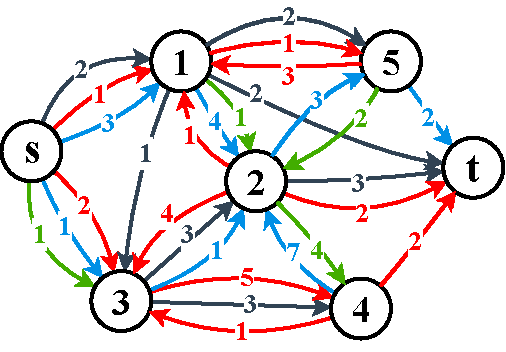
\includegraphics[scale=\scalefigure]{Figures/chap 3/Bold Filtered Graph.pdf}
%	\caption{The filtered graph $G'$}
%	\label{fig:filtered_graph}
%\end{figure}

\setlength{\intextsep}{3pt}
\renewcommand{\scalefigure}{0.7}
\begin{figure}[htbp]
	\centering
	\begin{subfigure}{.49\linewidth}
		\centering
		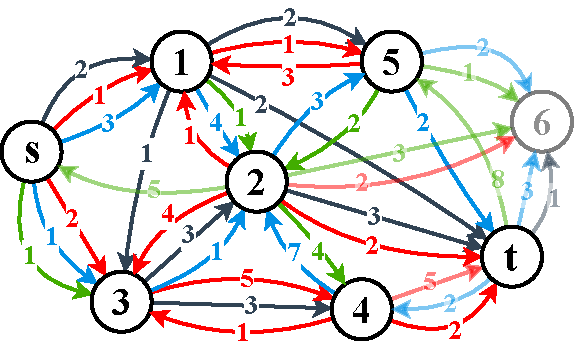
\includegraphics[scale=\scalefigure]{Figures/chap 3/Filtering Input Graph.pdf}
		\caption{The withdrawal of redundant edges and nodes}
		\label{fig:filteing_graph}
	\end{subfigure}
	\begin{subfigure}{.49\linewidth}
		\centering
		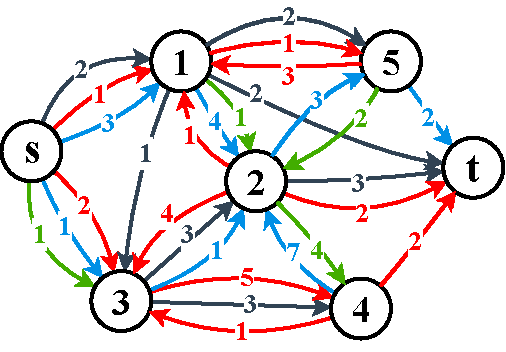
\includegraphics[scale=\scalefigure]{Figures/chap 3/Bold Filtered Graph.pdf}
		\caption{The filtered graph $G'$}
		\label{fig:filtered_graph}
	\end{subfigure}
	\caption{An example result of the pre-filtering process}
	\label{fig:filtering+process}
\end{figure}